\begin{figure}
  \centering
  \subfloat[]{%
    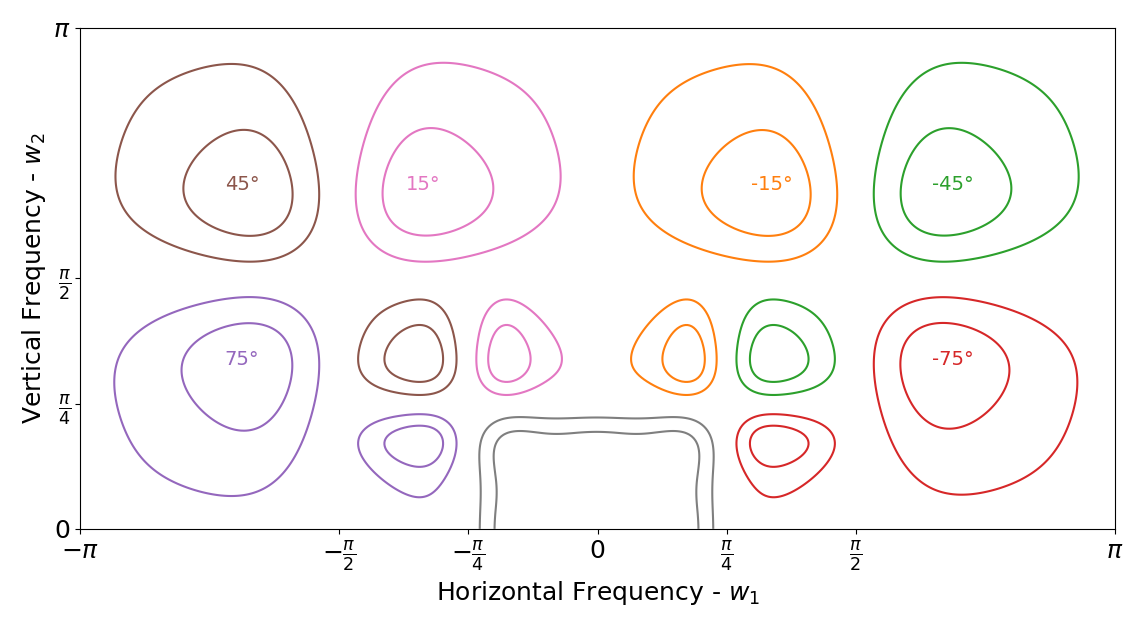
\includegraphics[height=6cm]{freqlearn/images/subbands.png}
    \label{fig:ch6:dtcwt_bands_freq}
  }
  \hspace{1cm}
%    \newline
  \subfloat[]{%
    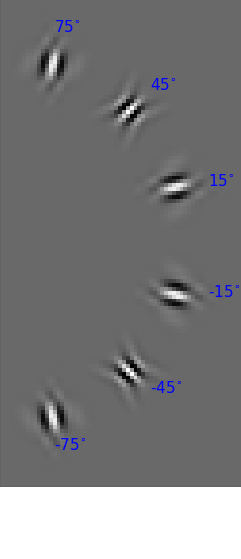
\includegraphics[height=5.7cm]{freqlearn/images/impulses.png}
    \label{fig:ch6:dtcwt_bands_impulse}
  }
  \mycaption{Contour Plots and Impulse Responses}{\subref{fig:ch6:dtcwt_bands_freq} Contour plots at
    -1dB and -3dB showing the support in the Fourier domain of the 6 subbands of
    the $\DTCWT$ at scales 1 and 2 and the scale 2 lowpass. These are the 
    product $P(z)Q(z)$ from \autoref{eq:ch6:end_to_end1}. 
    \subref{fig:ch6:dtcwt_bands_impulse} The pixel domain impulse responses for
    the second scale wavelets. } 
  \label{fig:ch6:dtcwt_bands}
\end{figure}
